\documentclass[12pt]{article}
%1inmargins
\usepackage[margin=1in,bottom=1in,top=1in]{geometry}
\usepackage{fancyhdr}
\usepackage{amsmath}
\usepackage{mathtools}
\usepackage{amssymb}
\usepackage{array}
\usepackage{tabu}
\usepackage{stmaryrd}
\usepackage{enumitem}
\usepackage{algpseudocode}
\usepackage{graphicx}
\graphicspath{ { ../fig/ } }
\pagestyle{fancy}
\lhead{\small Charlie Windolf}
\chead{\textbf{\textsf{Latent Structure Random Graphs (Draft)}}}
\rhead{\small Graphs and Networks}
\renewcommand{\headrulewidth}{0.4pt}
\setlength{\parindent}{24pt}
% independent RVs
\newcommand{\ind}{\protect\mathpalette{\protect\independenT}{\perp}}
\def\independenT#1#2{\mathrel{\rlap{$#1#2$}\mkern2mu{#1#2}}}
% nice parens
\newcommand{\lp}{\left(}
\newcommand{\rp}{\right)}
\newcommand{\rb}{\right]}
\newcommand{\lb}{\left[}
% handy
\newcommand{\R}{\mathbb{R}}
\newcommand{\iid}{\mathrm{iid}}
\newcommand{\C}{\mathbb{C}}
\newcommand{\E}{\mathbb{E}}
\renewcommand{\P}{\mathbb{P}}
\newcommand{\TV}{\mathrm{TV}}
\newcommand{\diag}{\mathrm{diag}}
% ugh
\newcommand{\bvi}[1]{\begin{psmallmatrix}X_{#1}\\Y_{#1}\end{psmallmatrix}}
\newcommand{\vv}[2]{\begin{psmallmatrix}#1\\#2\end{psmallmatrix}}
\newcommand{\vvv}[5]{\begin{psmallmatrix}#1\\#2\\#3\\#4\\#5\end{psmallmatrix}}
\newcommand{\bvvv}[5]{\begin{pmatrix}#1\\#2\\#3\\#4\\#5\end{pmatrix}}
\newcommand{\twotwo}[4]{\begin{psmallmatrix}#1 & #2\\#3 & #4\end{psmallmatrix}}
% complex sq
\newcommand{\bkkb}[2]{\braket{#1}{#2}\braket{#2}{#1}}
\newcommand{\bksq}[2]{\abs{\braket{#1}{#2}}^2}
% ez summation
\newcommand{\sumin}{\sum_{i=1}^n}
\newcommand{\lilsumin}{\Sigma_{i=1}^n}
\newcommand{\sumjn}{\sum_{j=1}^n}
\newcommand{\lilsumjn}{\Sigma_{j=1}^n}
\newcommand{\prodin}{\prod_{i=1}^n}
% Including Python
\usepackage[utf8]{inputenc}
\pagenumbering{arabic}
% \DeclareFixedFont{\ttb}{T1}{txtt}{bx}{n}{9} % for bold
% \DeclareFixedFont{\ttm}{T1}{txtt}{m}{n}{9}  % for normal
% Defining colors
\usepackage{xcolor}
\usepackage{courier}
\definecolor{deepblue}{rgb}{0,0,0.5}
\definecolor{deepred}{rgb}{0.6,0,0}
\definecolor{deepgreen}{rgb}{0,0.5,0}
\usepackage{listings}
% Python style for highlighting
\newcommand\pythonstyle{\lstset{
language=Python,
backgroundcolor=\color{white},
basicstyle=\ttfamily\scriptsize,
otherkeywords={self,as},            
keywordstyle=\color{gray}\textbf,
emph={__init__},
frame=tb,
emphstyle=\textbf\color{black},    
stringstyle=\color{gray},
commentstyle=\textcolor{gray},
showstringspaces=false            
}}
% Python environment
\lstnewenvironment{python}[1][]
{
\pythonstyle
\lstset{#1}
}
{}
\newcommand{\minor}{\ll}
\newcommand{\subdiv}{\sqsubseteq}
\newenvironment{alphenum}
    {\begin{adjustwidth}{-2em}{-2em}\begin{enumerate}[label={(\alph*)}]}
    {\end{enumerate}\end{adjustwidth}}
\newcommand{\sa}[1]{\begin{smashedalign}#1\end{smashedalign}\noindent}
\newcommand{\tdj}{\text{\dj}}
\DeclarePairedDelimiter\abs{\lvert}{\rvert}%
\DeclarePairedDelimiter\norm{\lVert}{\rVert}%
\DeclarePairedDelimiter\iverson{\llbracket}{\rrbracket}%
\makeatletter
\let\oldabs\abs
\def\abs{\@ifstar{\oldabs}{\oldabs*}}
\let\oldnorm\norm
\def\norm{\@ifstar{\oldnorm}{\oldnorm*}}
\makeatother
\newcommand*{\Value}{\frac{1}{2}x^2}%
\renewcommand\thesection{\textsf{\arabic{section}}}
\renewcommand\thesubsection{\textsf{\thesection.\arabic{subsection}}}
%%%%%%%%%%%%%%%%%%%%%%%%%%%%%%%%%%%%
\begin{document}

% \section{\textbf{\textsf{Abstract}}}

\section{\textbf{\textsf{Introduction}}}

\subsection{\textbf{\textsf{Random Geometric Graphs}}}

Random geometric graphs (RGGs) are a simple model for networks that form
according to the proximity of their vertices in space. They are discussed
in detail in Penrose \cite{mathewpenrose2003}, but briefly, an RGG
$G_{n, r}$ over $\{1,\dotsc,n\}$ can be constructed by choosing $n$ points
$U_1,\dotsc,U_n$ uniformly from the unit cube in a metric space with arbitrary dimension,
and then adding edges $\{i, j\}$ when $\norm{U_i - U_j} \leq r$. These graphs are
useful for studying real-world networks whose connections arise due to the physical
proximity of the nodes. One is displayed in Figure 1.

RGGs have been used to study the spread of computer viruses
on ad-hoc computer networks \cite{worm}, which are networks automatically formed
by a new class of devices that connect via short-range signals like WiFi and Bluetooth.
One can imagine a class of similar applications, such as the study of highway networks
or the electrical grid, or of any other sort of network that forms based on the
physical space in which it is situated.


\subsection{\textbf{\textsf{Generalizing RGGs}}}

A simple generalization of RGGs would be to remove the assumption that edges form
whenever nodes are closer than the threshold $r$. More generally, we can define
a generalized RGG $G_{n,f}$, parametrized by a function $f:\mathbb{R}^+_0\to[0,1]$,
again over the random points $U_1,\dotsc,U_n$, where edges $\{i, j\}$ appear
with probability $f(\norm{U_i - U_j})$. This model is strictly more general
than the one above, since a $G_{n,r}$ graph can be produced by choosing
$f(x)=\iverson{x\leq r}$, where the notation $\iverson{\mathrm{\textit{condition}}}$,
used throughout, indicates the function that is 1 when \textit{condition} is true
and 0 otherwise. This generalization allows for graphs whose edges form
with arbitrary probability according to the distance between two nodes:
maybe the're more likely to form when nodes are farther away, or according
to some probability distribution. Essentially any network that forms only
according to distances in physical space can be produced using this model.\par

\begin{figure}[t]
\begin{center}
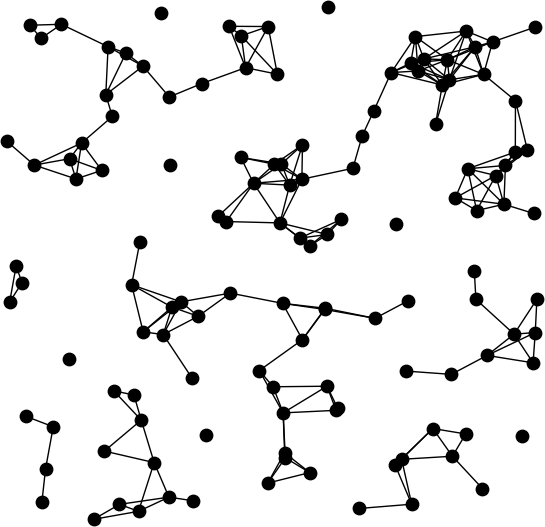
\includegraphics[width=200pt]{rgg}
\caption{An RGG generated with $n=128$, $r=0.1$.}
\end{center}
\end{figure} 

But we can imagine an even more general form, abstracting over the idea of
space. What if nodes connected not according to their geometric distance
from each other, but rather according to their separation in a graph? The
topology of a graph might be able to carry information about more general
structures than metric spaces. In general, such a model might be able to
describe connections that happen inside graphs: for example, it might be
able to predict networks of `likes' or `shares' that happen inside
social networks, or predict which members of a social network might
be likely to `friend' or `follow' each other given the current structure
of the social network. One could also imagine applications for recommender
systems: given a bipartite structure of users and, say, movies they have
watched, what users are likely to watch similar movies in the future?
Or, maybe such a model could predict which members of a nation's legislature
might be likely to collaborate on bills, given the structure of the legislature's
political hierarchy. In the following sections, we give a formalization
of such a model and study some of its properties.

\section{\textbf{\textsf{Latent Structure Random Graphs}}}

\subsection{\textbf{\textsf{Notation}}}

Jumping off of the above generalized RGGs, we propose a formalization
for random graphs produced using a probabilistic transformation
of a latent graph structure, which will be referred to as
Latent Structure Random Graphs (LSRGs). Formally, an LSRG $G_{L,f}$
is parametrized by a latent graph $L$ and a function
$f:\mathbb{Z}^+_0\to[0,1]$. We will let $G_{L,f}$ have the same vertices
as $L$, but edges $(i,j)$ in $G_{L,f}$ will each appear independently
with probability $f(\sigma_L(i, j))$, where $\sigma_L$ is the natural
distance metric associated with $L$. In the following remarks,
we will assume that $L$ and $G_{L,f}$ are simple graphs, possibly
with self-loops, for ease of analysis, although generalizations
to directed graphs with weighted edges should be apparent.\par

We will refer to the normalized degree distribution of $L$ as
$p=(p_0,p_1,\dotsc)$, with mean degree $c$. It will also be
helpful to name the normalized neighbor-degree distribution
$r=(r_0,r_1,\dotsc)$, indicating the distribution of the degrees
of vertices encountered after randomly choosing an edge and
following it to one of its endpoints. Let $c_r$ indicate the
mean neighbor-degree. When referring to $G_{L,f}$, let
$p'$, $c'$, $r'$, and $c_r'$ denote the corresponding entities.
Note that we may at times use $f_m$ to denote what should
properly be written $f(m)$, for brevity.


\subsection{\textbf{\textsf{Simple Case}}}

To get familiarized with this model, it will be helpful to
visualize a simple case, where $f$ is the point mass at 2,
e.g.\ $f(m) = \iverson{m = 2}$. The following figure will
show the sometimes surprising results of the LSRG model
for various latent structures $L$.\par

\begin{figure}[tp]
\begin{center}
\begin{tabular}{m{24pt} m{210pt}}
\textbf{\textsf{(A)}} & 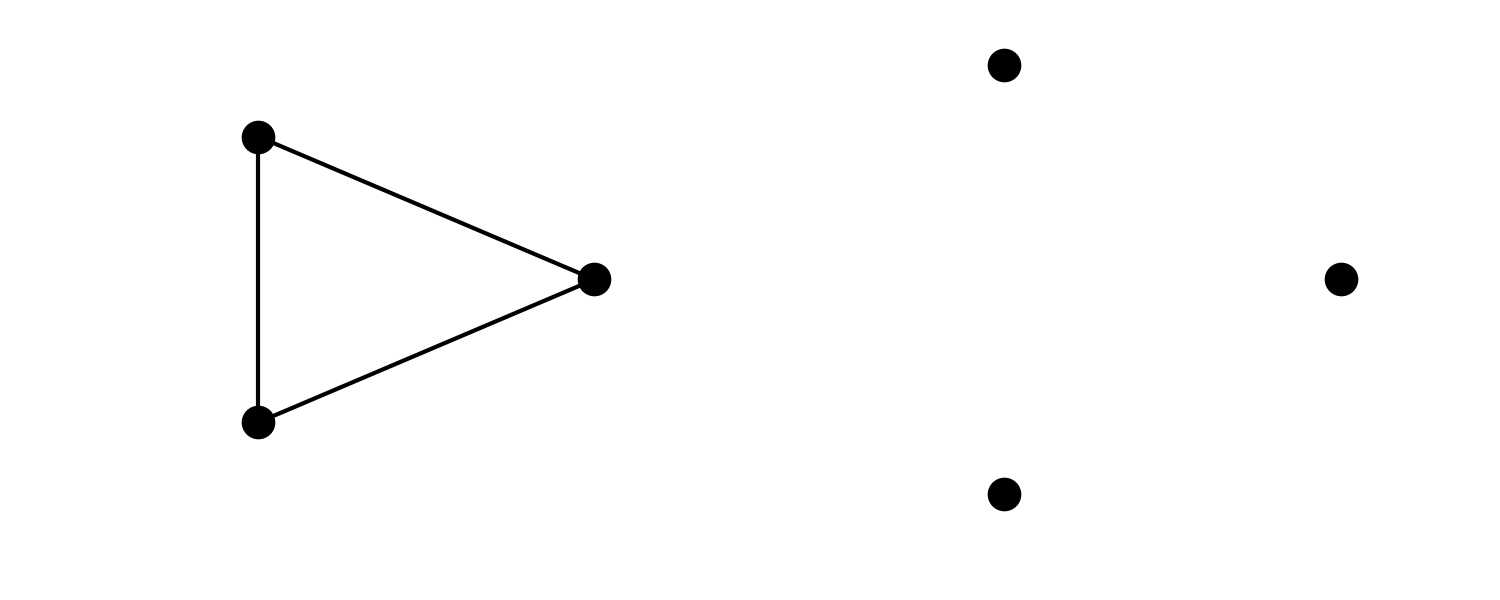
\includegraphics[width=200pt]{2_A.png} \\
\textbf{\textsf{(B)}} & 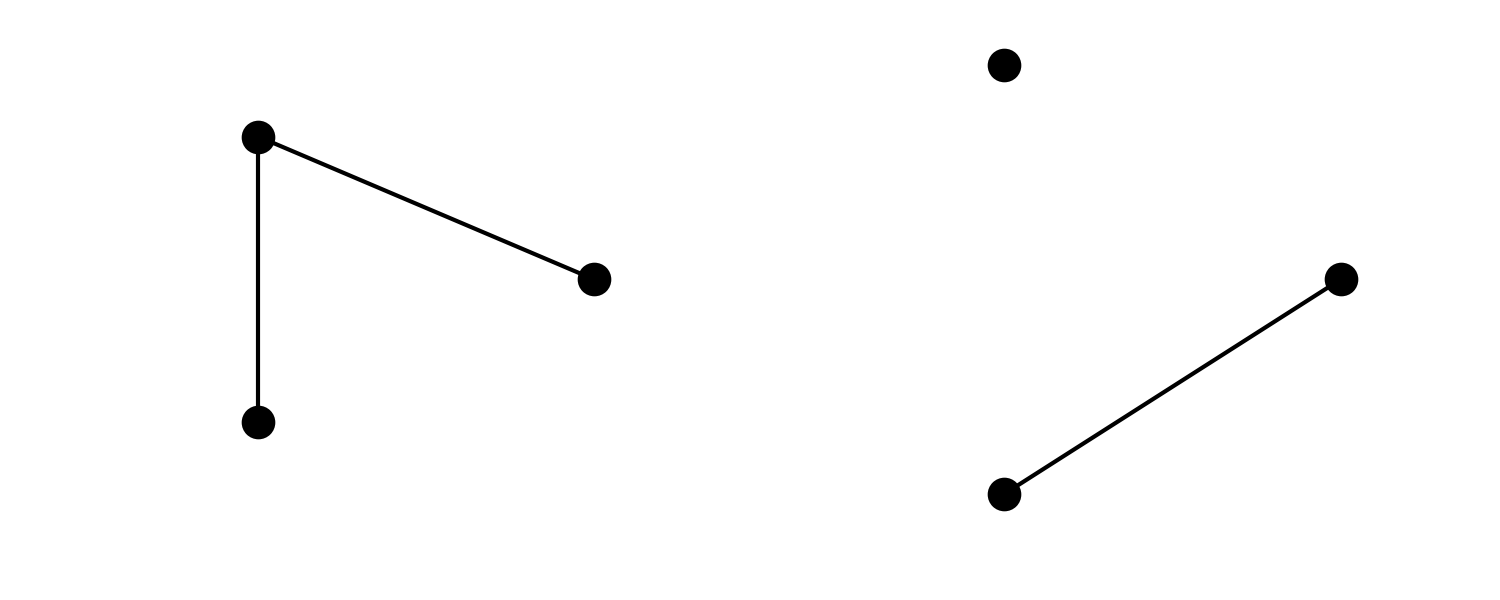
\includegraphics[width=200pt]{2_B.png} \\
\textbf{\textsf{(C)}} & 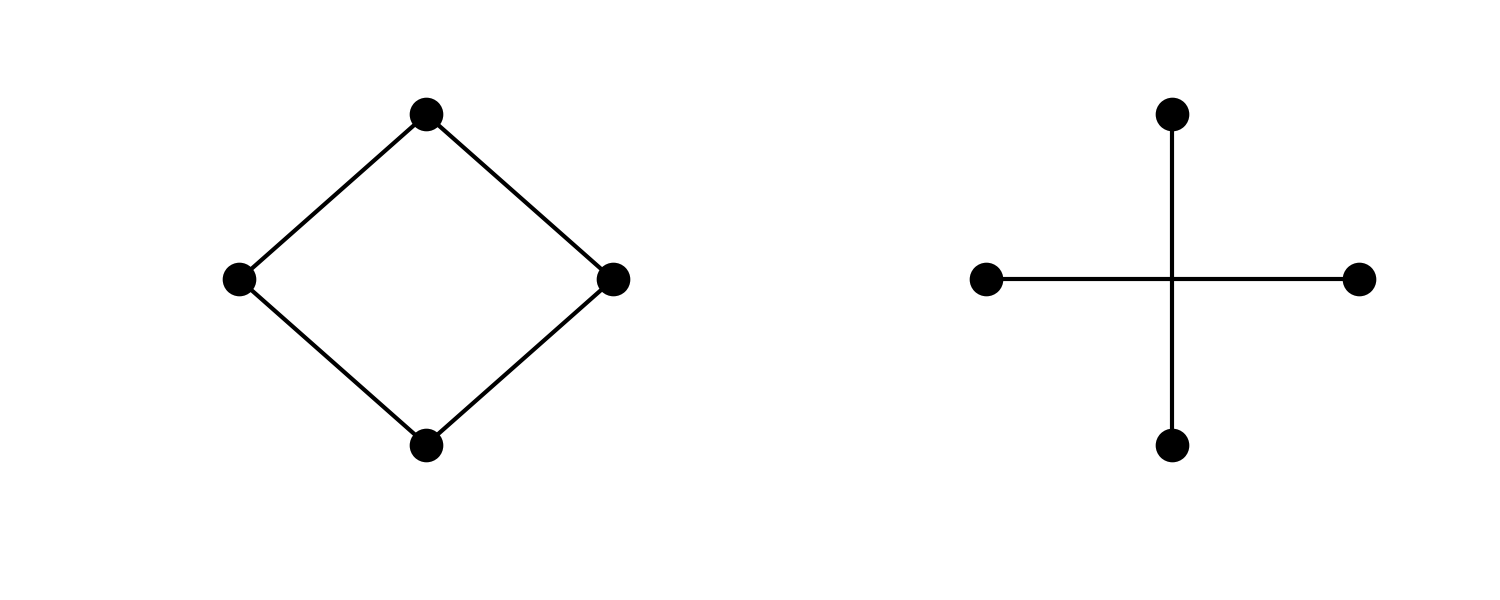
\includegraphics[width=200pt]{2_C.png} \\
\textbf{\textsf{(D)}} & 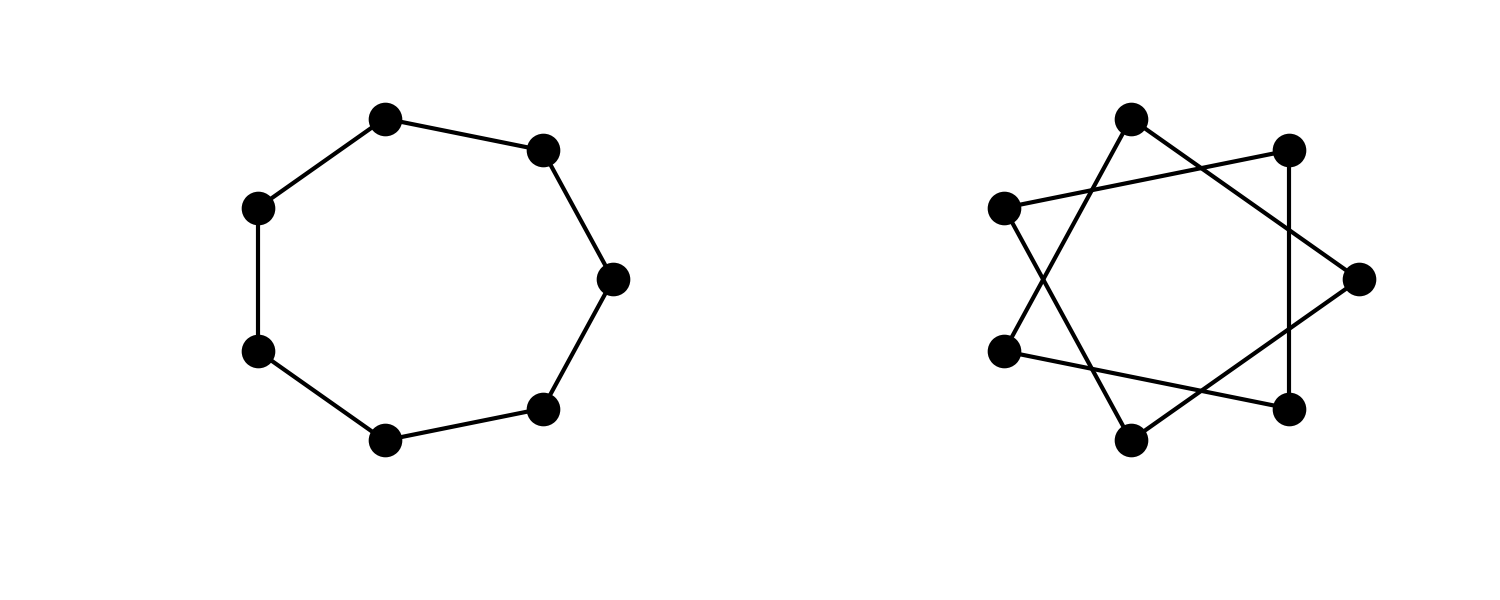
\includegraphics[width=200pt]{2_D.png} \\
\textbf{\textsf{(E)}} & 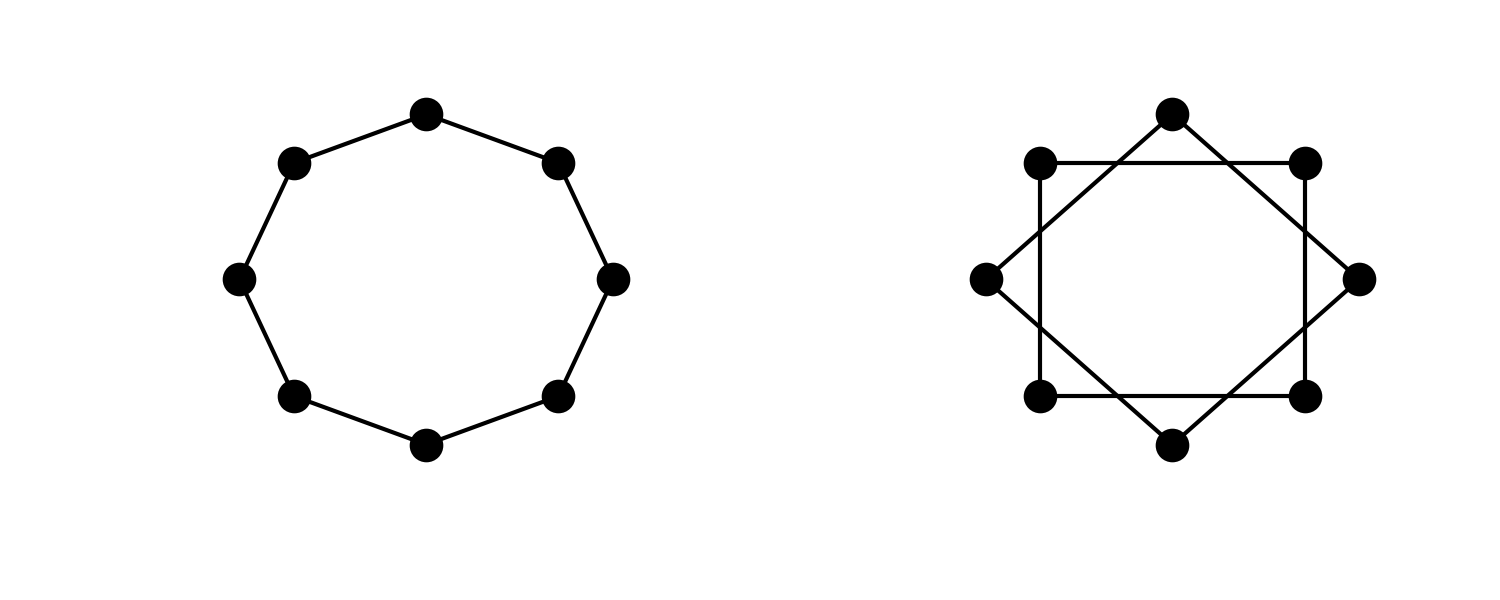
\includegraphics[width=200pt]{2_E.png} \\
\textbf{\textsf{(F)}} & 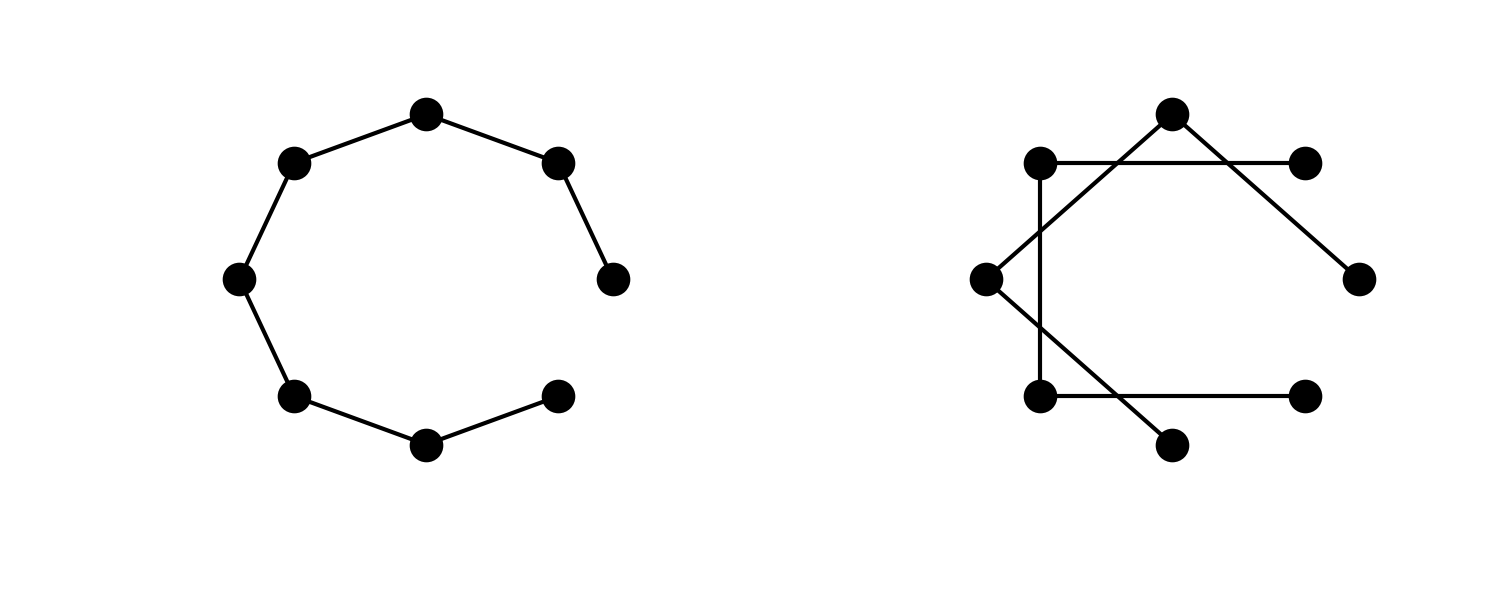
\includegraphics[width=200pt]{2_F.png}
\end{tabular}
\caption{The result of the LSRG model with $f(m)=\iverson{m=2}$ on
some small graphs. Latent graphs appear on the left, and their
corresponding LSRGs are on the right.}
\end{center}
\end{figure}

Even for such simple $f$ and $L$, the model produces some interesting
results that interact closely with the underlying latent structure.
For graphs of very low order (A-C), it produces the edge complement of the
latent graph. For cycle graphs (D-E), it produces an isomorphic cycle
when the number of vertices is odd (D), or two isomorphic cycles when
the number of vertices is even. For path graphs (F), it `unzips' the
path into two separate paths. From these examples, we can see that this
model is capable of producing the $k$-fuzz \cite{doylesnell} of $L$
by choosing $f(m)=\iverson{1 \leq m \leq k}$, and that in general, it
produces a probabilistic variant on the idea of the $k$-fuzz, allowing
for more general structures to form and building in randomness.
We will continue with the simple $f(m)=\iverson{m=2}$ case in the next
section to get a feel for how LSRGs behave with more complex latent
graphs.


\section{\textbf{\textsf{Motivating Example}}}

\subsection{\textbf{\textsf{Preferential Attachment Graphs}}}

Since this model is meant to describe phenomena arising on real-world
networks, it makes sense to study it using a latent graph with real-world
structure. Two candidates are the preferential attachment model proposed by
Barab{\'a}si and Albert \cite{prefatt} and D.~J. de Solla Price's cumulative
advantage model \cite{cumadv}. Both of these models attempt to explain the
growth of real-world networks in terms of `rich get richer' phenomena,
and have proposed as suitable for the study of social networks, technological
networks, and others. A more in depth comparison of the two appears in
Newman \cite{Newman2003}, but for now, it might make sense to begin with
the simpler preferential attachment model and see if it can be used
productively.\par

A preferential attachment graph $G_{n,c}$ is recursively grown, starting
from some inital graph, and adding new nodes one at a time. Each new node
gets $c$ edges, which connect to already existing nodes with probability
proportional to their degree. This process results in graphs with the
so-called `scale-free' property of having a degree distribution with
a power-law tail, and intuitively exposes a possible mechanism for the
presence of that sort of scaling in real-world systems. We will consider
the $f$ discussed above, and attempt to see what properties we can compute
for $G_{L,f}$ when $L$ is a tree generated by preferential attachment.


\subsection{\textbf{\textsf{Simple Case, Revisited}}}

We would like to study the case where $L$ is a preferential attachment
graph with $c=1$, which naturally produces recursive trees, in the
limit as $n$ grows. Finding properties of LSRGs produced from such $L$
in the special case $f(m)=\iverson{m=2}$ reduces to characterizing
the grandchildren of a given node when that node is considered the
root of the tree. For example, the mean degree $c'$ of $G_{L,f}$ is simply
the expected number of grandchildren of a random node in $L$.\par

To find $c'$, we will need to use certain facts about $L$.
Preferential attachment graphs are well studied, and in particular,
results for the degree distribution $p$ in the limit of large $n$ have
been obtained, taking the form $p_k \sim k^{-3}$
in the limit of large $k$, or more precisely
\[
p_k = \frac{2c(c+1)}{k(k+1)(k+2)}\ ,
\]
as shown by Bollob{\'a}s et.\ al.\ \cite{bollobas}. When $c=1$,
that comes out to
\[
p_k = \frac{4}{k(k+1)(k+2)}\ .
\]
Additionally,
Fotouhi and Rabbat \cite{fotouhi} have given an expression for the
normalized conditional degree distribution $p(\ell\mid k)$, which
denotes the probability that a random neighbor of a node with
degree $k$ will have degree $\ell$, which in the $c=1$ case is
given by
\[
p(\ell\mid k) = \frac{k+2}{k\ell(\ell + 1)} - \frac{6}{k\ell}
\frac{{{k + \ell - 2}\choose{\ell - 1}}}{{{k + \ell + 2}\choose \ell}}\ .
\]
Since the degree of a node in $G_{L,f}$ is its number of grandchildren
in $L$, we ought to be able to use the above to solve for $G_{L,f}$'s
degree distribution. To find that distribution $p'$, we can use
the law of total probability:
\begin{align*}
p'_i &= \P(\text{random }v\in V(L)\text{ has }i\text{ granchildren})\\
     &= \sum_{k=0}^\infty p(i \mid k)p_k
\end{align*}
This procedure could be carried out in practice for real-world observed
graphs, but it is clearly not a general enough method for use in most
cases. Even in this case, where $f$'s support is very small, evaluating
this sum analytically would be hard, and won't generalize to different
$f$. So, from this example we can infer that we have a need for better
tools.\par

We can also get a hint that the preferential attachment model
might not be the best one to use by attempting to calculate the
expected conditional degree. In the following, let $D_i$ be the random
variable denoting the degree of vertex $i$ in $G_{L,f}$, and $d_i$
be $i$'s degree in $L$. Then we can say
\begin{align*}
\E[D_i \mid d_i=k] &= k \sum_{\ell=0}^\infty (\ell\,p(\ell\mid k) - 1)\ ,
\end{align*}
because once we know $d_i=k$, $D_i$ will be given by the the degrees
of $i$'s $k$ neighbors. But, substituting our expression for $p(\ell\mid k)$,
we can see immediately that this sum diverges because of $p(\ell\mid k)$'s
heavy tails. In other words, in the limit of large $n$, there might
exist a node that will connect to a substantial fraction of the rest
of the graph. In Fig.\ 3, this effect is shown on a small graph.
The dense center of the preferential attachment tree, filled with nodes
whose degrees are in the heavy tail of its degree distribution, becomes a
tangled web of edges since each has so many neighbors of neighbors.\par

\begin{figure}[t]
\begin{center}
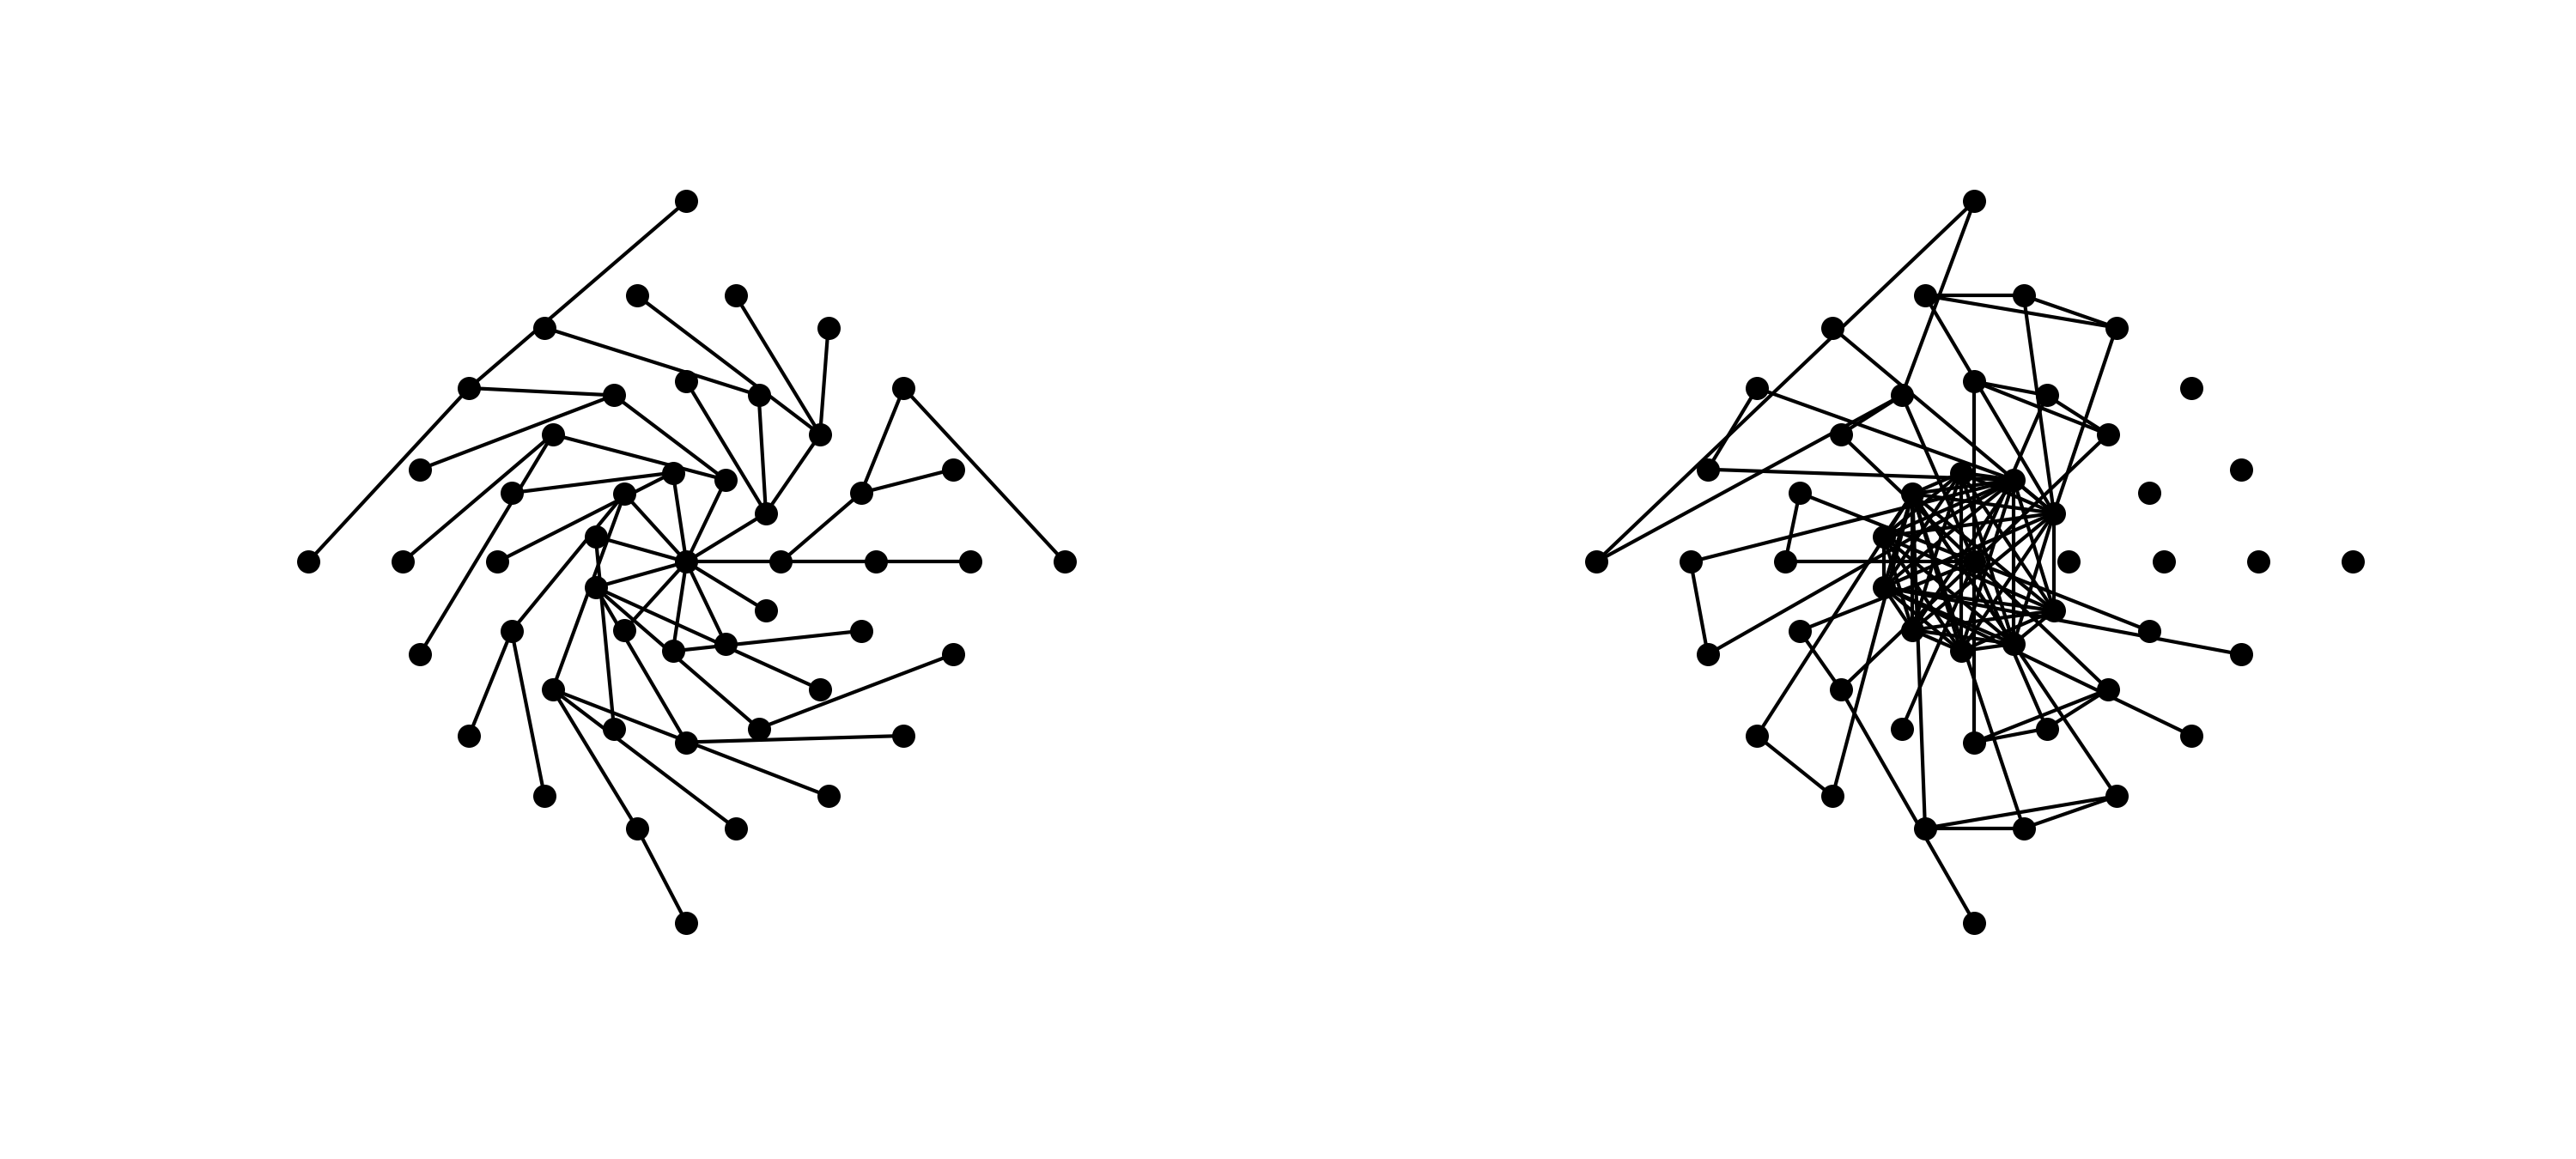
\includegraphics[width=300pt]{3}
\caption{An LSRG $G_{L,f}$ (right) where $f(m)=\iverson{m=2}$ and $L$ (left) is a
tree generated by preferential attachment $n=50$.}
\end{center}
\end{figure}


The problem is that the Barab{\'a}si and Albert model produces graphs with
too-heavy tails, which cannot be adjusted. Luckily, Price's cumulative
advantage model provides a way to adjust the decay rate of its asymptotic
degree distribution, while still retaining scale-free structure.

\subsection{\textbf{\textsf{Cumulative Advantage Graphs}}}

In what follows, we will make use of a slightly modified version of
Price's cumulative advantage model. The main differences are that we
will erase edge directions once the graph is grown, and that the out-degree
of nodes is fixed instead of random. To construct such a graph $G_{n,\alpha,c}$,
after choosing a smoothing parameter $\alpha$ and an out-degree $c$, and
starting from some initial graph, recursively add nodes. After a node has been
added, add edges from it to $c$ other nodes, where the other nodes
are selected independently with probability
\[
\frac{d^{\text{(in)}}_i + \alpha}{n(\bar{d}^\text{(in)} + \alpha)}\ ,
\]
which is the add-$\alpha$ smoothed version of the Barab{\'a}si-Albert
process. Once the graph is constructed, erase edge directions. Again,
setting $c=1$ produces trees.\par

These graphs are also relatively well studied. As Price showed,
in the limit of large $n$ and when $c=1$, their in-degree distribution
looks like
\[
p_k = \frac{\alpha + 1}{2\alpha + 1}\prod_{j=1}^{k-1}\frac{\alpha - 1 + j}{2\alpha + 1 + j}\ ,
\]
which looks like $p_k \sim k^{-2-\alpha}$ as $k$ grows. However,
there seems to be no expression like for the conditional degree
distribution, like there was above. Without that information,
we will have to use new tools, which are developed in the next section.


\section{\textbf{\textsf{Degree Properties and Generating Functions}}}

\subsection{\textbf{\textsf{Molloy and Reed Random Graphs}}}

Since we have no information about the conditional degree distribution of Price's model
graphs, it makes sense to assume that for any neighbors $i,j\in V(L)$, their degrees
are independent. This setup is equivalent to assuming that we are working with
graphs selected uniformly at random from all graphs with $L$'s degree sequence,
or in other words, the generalized random graphs studied by Molloy and Reed \cite{molloy95,molloy98}.
These graphs are as random as possible given their degree sequence, meaning that
edges appear independently once it is known. Our procedure will be to generate
Price trees with $\alpha=2$, to get a degree distribution whose tails decay
sufficiently quickly, and then to generate a Molloy and Reed random graph
over the tree's degree sequence. To keep the graph connected and aid analysis,
we will take just the giant component from that random graph, and use it
as the latent graph $L$ to be fed into our model. Figure 4 compares the
degree distributions of the $G_{L,f}$ that result when doing this procedure
and using the tree from Price's model without going through the Molloy and
Reed graph.

\begin{figure}[t]
\begin{center}
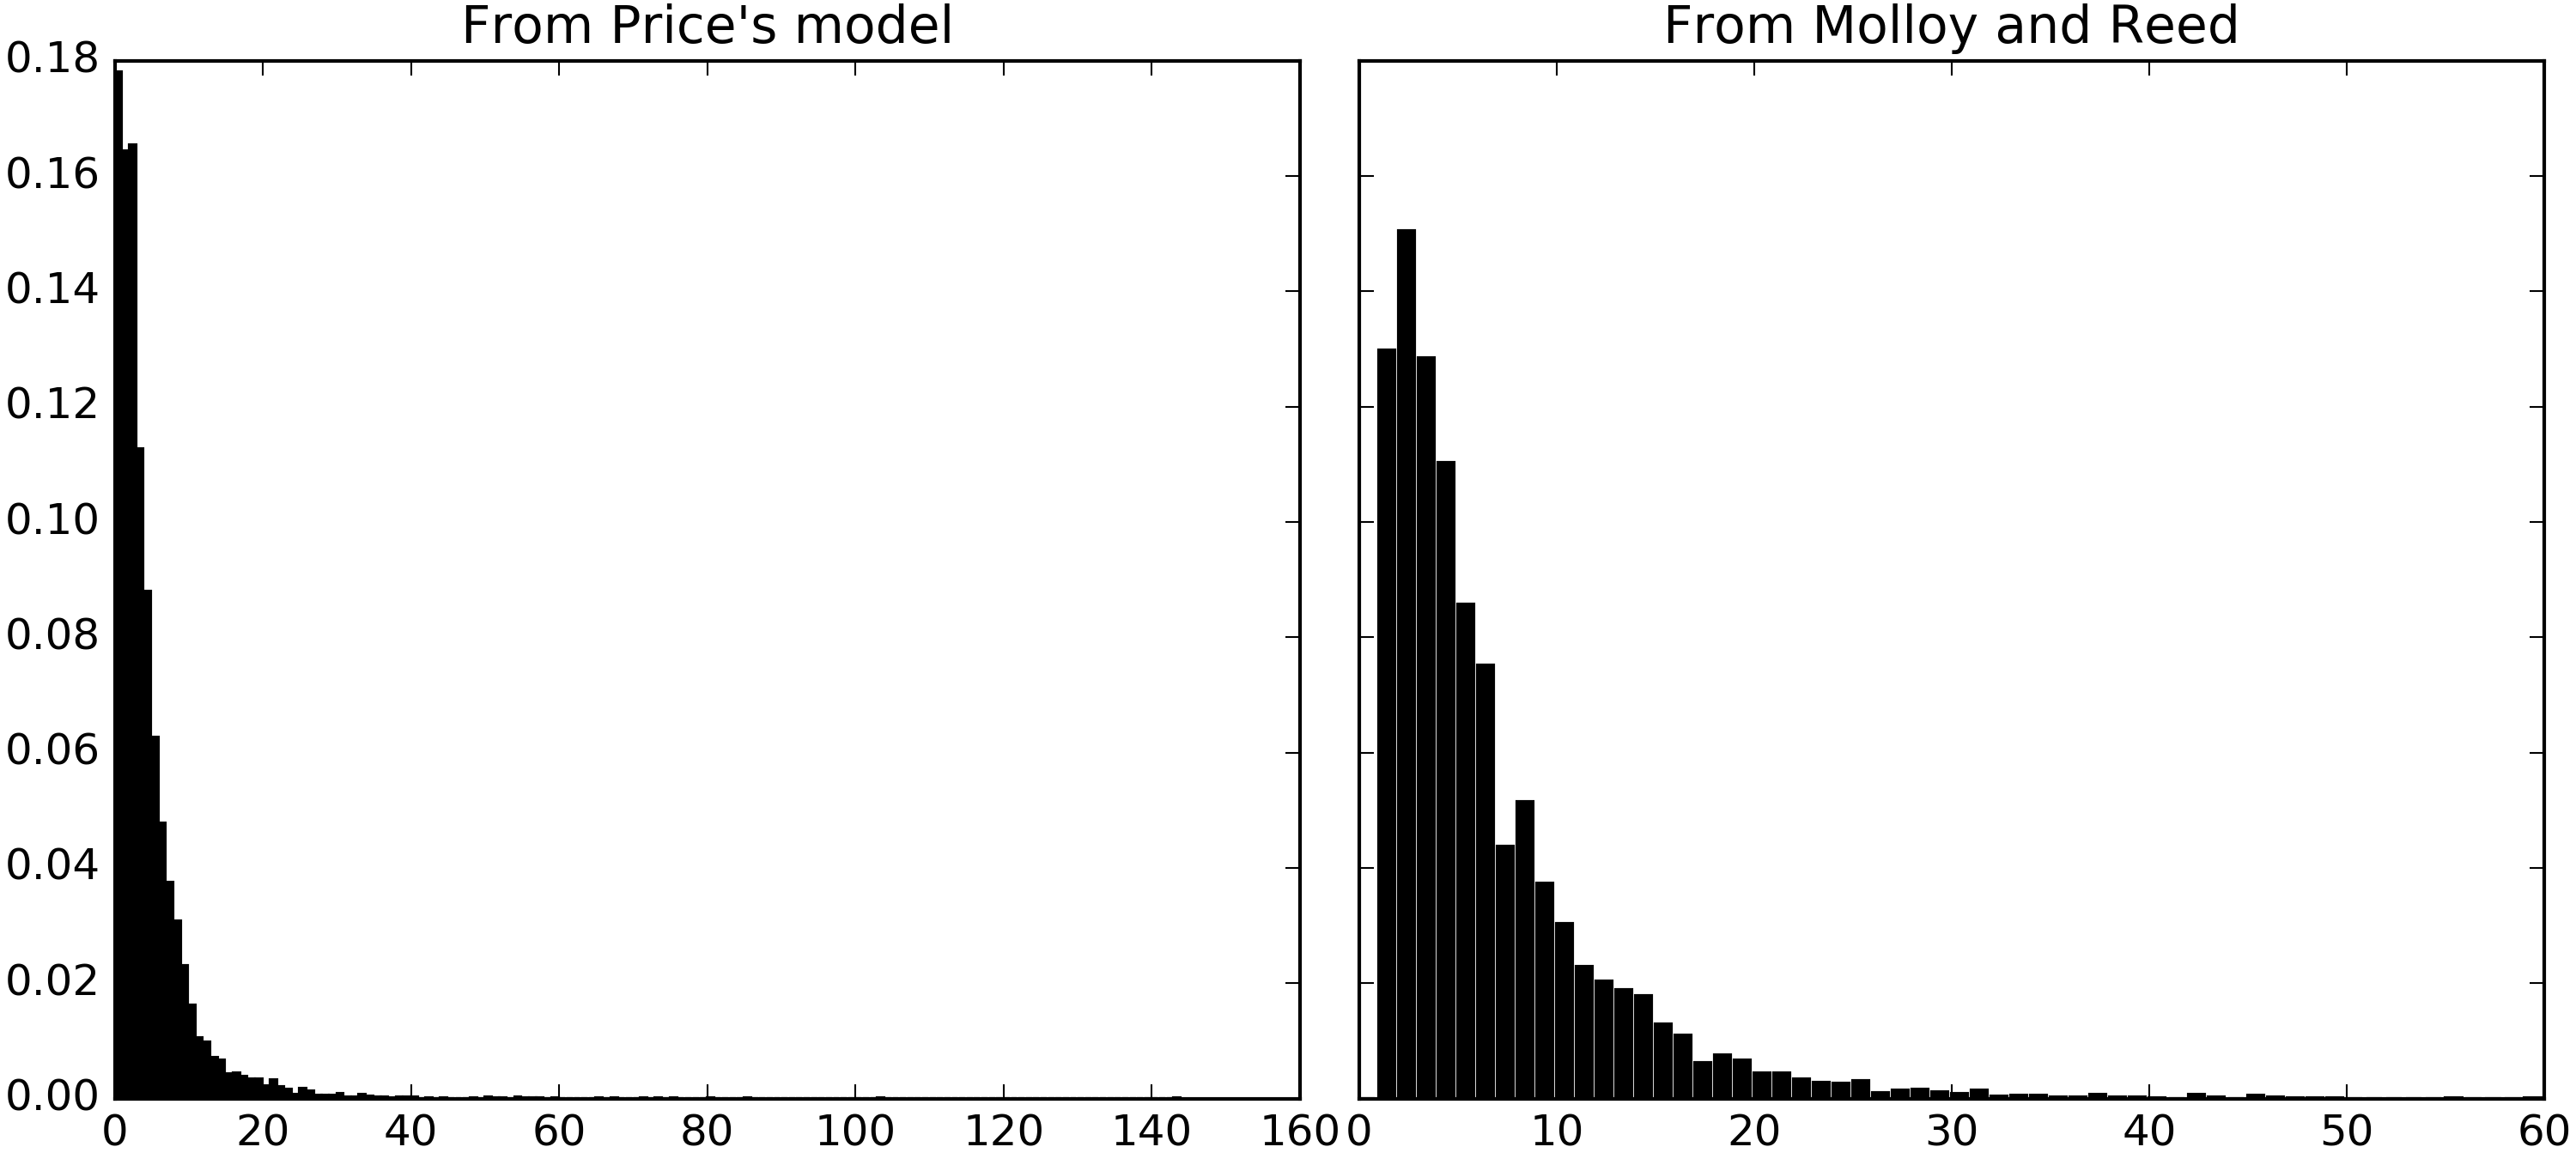
\includegraphics[width=300pt]{4}
\caption{Degree distributions for $G_{L,f}$ where $f=\iverson{m=2}$. On the left,
$L$ is a tree generated with Price's model. On the right, $L$ is the giant
component of a Molloy and Reed random graph generated from the Price tree's
degree sequence. Both have $n=10,000$. Because it is only the giant component, there are no zero-degree
nodes and significantly fewer low-degree nodes, but the middle sections of these
two pmfs are comparable.}
\end{center}
\end{figure}


\subsection{\textbf{\textsf{Probability Generating Functions and Branching Processes}}}

In the Molloy and Reed setting, many useful tools become available, among them the
formalization of branching processes and probability generating functions, for
instance as they are used in Newman \textit{et.\ al.} \cite{newman01} in the study
of cluster growth. In that paper, the authors study the random variable representing the
size of the component in which a random node resides. Let $Z$ be the random variable
describing this quantity, and let $v$ be the random node in question. The authors
study component size by imagining component growth as a branching process starting at $v$.
Let $Z_m$ refer to the (random) number of children in the $m$th generation of the branching process.
Then, he zeroth generation of the branching process always has one node, namely $v$, giving
$Z_0 = 1$. The first generation consists of $v$'s neighbors. Since $v$ is a random node, that means
that $Z_1$ is distributed according to the pmf $p$. The second generation consists of $Z_1$ branches,
each of which will produce a number of children drawn from the graph's neighbor-degree pmf,
which we called $r$. In the Molloy and Reed setting, $r$ can be shown to be given by
\[ r_k = \frac{k+1}{c}p_{k+1}\ . \]
Subsequent generations of the branching process also have the number of children in each
of their branches drawn from $r$. Our goal is to study the $Z_m$ and see if we can
figure out how many neighbors $v$ will have in $G_{L,f}$ given $f(m)$ and $Z_m$.\par

To do so, we will make some use of generating functions. Here, we will introduce some
of the properties of generating functions that were the most useful in this work,
but we direct interested readers to Wilf's thorough text \cite{wilf}. For any
pmf $a=(a_0,a_1,\dotsc)$, we say that $a$ is `generated' by the function
\[g_a(s) = \sum_{i=0}^\infty a_k s^k\ , \]
because we can take derivatives to find that the probability $a_k$ is given
by
\[ a_k = \frac{1}{k!}{g^{(k)}_a(0)}\ , \]
where $g^{(k)}_a(s)$ denotes the $k$th derivative of $g_a$ with respect to $s$.
We will also sometimes say that $g_a$ generates random variables $A$ distributed
according to $a$, and refer to $g_a$ as $g_A$.
Note also that since $a$ is a pmf, $g_a(1)=1$. Additionally, taking a single
derivative and evaluating at $s=1$ gives
\[ \left.g'_a(s)\right\rvert_{s=1} = \left.\sum_{k=1}^\infty k a_k s^{k-1} \right\rvert_{s=1} = \sum_{k=0}^\infty k a_k\ , \]
which is exactly the expected value of a random variable distributed according to $a$.
The last and most interesting property of pgfs that we will use here is
that for arbitrarily distributed and independent random variables
$N$ and $X_1,X_2,\dotsc \thicksim_\iid$, where $N$ is generated by $g_N$ and
the $X_i$ are all generated by the same pgf $g_X$, the random variable
\[ S = \sum_{i=1}^N X_i \]
is generated by the composition of $g_N$ and $g_X$, e.g. \[ g_S(S) = g_N(g_X(S))\ . \]
In the following, we will use $\circ$ to denote function composition, and let
$g_a^n$ be $g_a \circ g_a \circ \dotsm \circ g_a$, $n$ times. For convenience,
we will say that $g_a^0$ is the identity function, which turns out to
generate the point mass pmf centered at 1.\par

With this notation in place, we can elaborate on the study of component growth
presented in \cite{newman01}. It will be useful for us to understand
what the generating functions $g_{Z_m}$ of the generations $Z_m$ are
in order to understand the structure of our latent structure graphs.
First, note that since there is always one node in the zeroth generation,
it is simply generated by the identity function $g_{Z_0}(s) = s$.
Since $Z_1 \thicksim$ pmf $p$, $g_{Z_1} = g_p$. From this point on,
the size of a future generation $Z_m$ is determined by $Z_{m-1}$
branches, each of which independently realizes some children
according to $r$. In other words, if $N_1, N_2, \dotsc$ are
independent random variables distributed according to $r$, then
\[ Z_m = \sum_{i=1}^{Z_{m-1}} N_i. \] So, we can use the property
of generating functions described above, which gives the recurrence
relation \[ g_{Z_m} = g_{Z_{m-1}} \circ g_r. \] This relation
is easily solved given the initial conditions above, yielding
\[ g_{Z_m} = g_p \circ g_r^{m - 1}. \]
Here, we can compute the expected number of nodes in any generation,
$\E[Z_m]=g_{Z_m}'(1)$,
starting with the first few, after which a pattern will become apparent.
\begin{align*}
g_{Z_1}'(s) &= g_p'(1) = c \\
g_{Z_2}'(s) &= g_p'(g_r(1))g_r'(1) = c_r c \\
g_{Z_3}'(s) &= g_p'(g_r^2(1))g_r'(g_r(1))g_r'(1) = c_r^2 c
\end{align*}
In general, we can see that the chain rule for differentiation will
produce
\[ \E[Z_m] = c_r^{m-1}c\ , \]
which for large $m$ will always either go to zero or diverge to infinity,
depending on the value of $c_r$. At this point,
we have laid the groundwork for further investigation of LSRGs.

\subsection{\textbf{\textsf{Degree Properties of LSRGs}}}

We can think of a random node $v$'s degree $D_v$ in $G_{L,f}$ similarly
to how we think of the growth of $v$'s component, in terms of a branching
process. The analogy works because $v$ might have an edge to each of the nodes
in the $m$th generation of the branching process, independently with probability
$f(m)$. So, removing the randomness associated with $f$, $D_v$ is completely
determined by the $Z_m$.\par

Let $D_{v,m}$ be the random variable indicating how many neighbors $v$ gets
in $G_{L,f}$ from the $m$th generation of the branching process, or in other
words, the number of $v$'s neighbors in $G_{L,f}$ that were distance $m$ from
$v$ in $L$. There will be $Z_m$ candidates, each of which is accepted
or rejected according to a coin toss with probability $f(m)$. So, we
can describe $D_{v,m}$ by introducing new random variables for the
possible edges $E_{m,1}, E_{m,2},\dotsc \thicksim_\iid$ Ber$(f(m))$, which
gives \[ D_{v,m} = \sum_{i=0}^{Z_m} E_{m,i}.\] We can use our composition
trick again to obtain \[ g_{D_{v,m}} = g_{Z_m} \circ g_{E_{m}}, \]
where $g_{E_m}$ is the well known generating function for Bernoulli
random variables \[ g_{E_m}(s) = 1 - f(m) + f(m) s\ . \]\par

At this point, even without solving for $g_{D_v}$, we can already
estimate its expected value. Applying linearity of expectation and using
the pgf expression for expected value, we can write
\begin{align*}
\E[D_v] &= \sum_{m=0}^\infty \E[D_{v,m}] \\
        &= \sum_{m=0}^\infty g_{D_{v,m}}'(1) \\
        &= \sum_{m=0}^\infty g_{Z_m}'(g_{E_m}'(1))g_{E_m}'(1)
\end{align*}
Here, pause to note that $g_{E_m}'(1) = f(m)$, which leaves
\begin{align*}
\E[D_v] &= \sum_{m=0}^\infty g'_{Z_m}(1) f(m) \\
        &= \sum_{m=0}^\infty c_r^m c f(m) \\
        &= c \sum_{m=0}^\infty c_r^{m-1} f(m) \\
        &= \frac{c}{c_r} g_f(c_r)\ .
\end{align*}
Note that $g_f$ is not a probability generating function, but just the
regular generating function for the sequence $f=(f(0),f(1),\dotsc)$.
This brief expression says a good deal about the behavior of our model,
in large part because it shows what kind of $f$ will be `well-behaved'
for a given $L$, using the well-developed theory of convergence and
infinite series. For $c_r<1$, $f$ does not have to decay so quickly,
but for $c_r > 1$, which is the situation we are interested in,
we need $f$ to drop off very fast indeed. We are concerned with the
$c_r > 1$ case because it corresponds to a supercritical branching process
for component growth, and we are studying the giant component of a graph,
which indicates that the process would have to be supercritical.
Note that $c_r$ can be expressed simply in terms of generating functions,
with $c_r = \frac{g_p''(1)}{g_p'(1)}$.\par


\subsection{\textbf{\textsf{Notes on Simulation}}}

hi


\section{\textbf{\textsf{Degree Properties with Convolution Approach}}}

\subsection{\textbf{\textsf{Branching as Convolution}}}

We begin this alternate approach with a reexpression of the branching
process above in terms of convolutions of random variables. Recall that
$Z_0,Z_1,\dotsc$ indicate the random quantities of nodes at each level
of the branching process, and that $Z_0=1$, $Z_1$ is drawn from $p$,
and that for $m>1$, $Z_m$ is built from $Z_{m-1}$ iid samples from $r$.
Let $z_0,z_1,\dotsc$ be the pmfs for these random variables. We can
observe that $z_0$ is the point pmf at 1, and that $z_1 = p$. From these
initial conditions, $z_m$ can be specified recursively, given $z_{m-1}$
and for $m>1$ as follows, using the law of total probability:
\[
z_m(i) = \sum_{j=0}^\infty \P(Z_m=i\mid Z_{m-1}=j)\P(Z_{m-1}=j)\ .
\]
But recall that given $Z_{m-1}=k$, $Z_m$ is the sum of $j$
random variables $R_1,\dotsc,R_j \thicksim_\iid r$. So, we can calculate
the pmf of the sum of these random variables by the $j$-fold convolution
of their pmf $r$. Let $r^j(i)$ denote the probability that this sum equals
$i$. Then we can write
\[
z_m(i) = \sum_{j=0}^\infty r^j(i)z_{m-1}(j)\ ,
\]
after substituting $z_{m-1}(j)$ for $\P(Z_{m-1}=j)$.\par

Having the pmfs $z_m$ is helpful, but even better would be to have a pmf for
the total $Z=\sum_m Z_m$. To do so, it will be helpful to observe that
when calculating $\P(Z=k)$, only the first $k$ generations matter. $Z_0$
is always 1, and if a $Z_m$ is ever 0, the branching process has to stop.
That means that to accumulate $Z=k$, it will take at most $k$ generations,
summing from $Z_0$ out to $Z_{k-1}$, as long as $Z_k=0$. It will help to
introduce some notation. Let \[ T_k = \sum_{m=0}^{k} Z_m \] indicate the
total size of the branching process out to generation $k$, and define
\[ \tau_m(i, j) = \P(Z_m = i, T_m = j)\ .\] Then, by the argument above,
we can write \[ \P(Z = k) = \P(Z_k=0,T_k=k) = \tau_k(0,k)\ . \]\par

With this formalization in place, we can go back to LSRGs with some idea
of where we will be heading.

\subsection{\textbf{\textsf{LSRGs with Convolution}}}

As we observed earlier, given that $Z_m=j$, $D_{v, m}$ becomes a sum of
$j$ iid Bernoulli random variables, each with success probability $f_m\equiv f(m)$.
In other words, the following conditional pmf is that of a Binomial random
variable: \[ \P(D_{v,m} = k \mid Z_m = j) = {j \choose k} f_m^k(1-f_m)^{j-k}\ .\]
This relation is helpful, because we have the pmfs for each $Z_m$ from above.
That means that we can use the law of total probability again, to define the
new sequence of pmfs
\begin{align*}
d_m(k) &\equiv \P(D_m=k) \\
       &= \sum_{j=0}^\infty \P(D_{v,m}=k \mid Z_m = j)\P(Z_m=j)\\
       &= \sum_{j=0}^\infty {j \choose k} f_m^k(1-f_m)^{j-k} u_m(j)\ .
\end{align*}\par
With these results in place, we can begin to calculate the pmf\[d(k)\equiv \P(D_v = k)\ .\]
Building off of the random variables $T_m$ defined above, define new random
variables $U_0,U_1,\dotsc$ like \[U_m = \sum_{k=0}^m \sum_{\ell=1}^{Z_k} E_{m,\ell}\ ,\]
where $E_{m,\ell}\thicksim_\iid \text{Bernoulli}(f_m)$ as above. Also, let
\[ \omega_m(i, j)=\P(Z_m=i, U_m=j)\ .\] Thanks to the Markovity of $Z_{m+1}$ given
$Z_m$, this expression yields the following recurrence for $\omega_{m+1}$, 
by the law of total probability:
\begin{align*}
\omega_{m+1}(i,j)&=\P(Z_{m+1}=i, U_{m+1}=j)\\
&= \sum_{k=0}^\infty \sum_{\ell=0}^\infty \P(Z_{m+1}=i,U_{m+1}=j\mid Z_m=k, U_m=\ell)\,\P(Z_m=k,U_m=\ell)\\
&= \sum_{k=0}^\infty\sum_{\ell=0}^\infty \P(U_{m+1}=j\mid U_m=\ell,Z_{m+1}=i)\,\P(Z_{m+1}=i\mid Z_m=k)\,\omega_m(k,\ell) \\
&= \sum_{k=0}^\infty\sum_{\ell=0}^\infty \P(U_{m+1}=j\mid Z_{m+1}=i)\,r^\ell(j)\,\omega_m(k,\ell) \\
&= \sum_{k=0}^\infty\sum_{\ell=0}^\infty \binom{i}{j} f_m^i (1 - f_m)^{j-i}\,r^\ell(j)\,\omega_m(k,\ell) \ .
\end{align*}
To justify the above, note that the third and fourth steps follows from the second by substituting
$\omega_m$ for the joint distribution of $Z_m$ and $U_m$, and by breaking the joint
distribution of $Z_{m+1},U_{m+1}$ when conditioned on $Z_m,U_m$ up using the fact that
$U_{m+1}$ only depends on $Z_{m+1}$ and $Z_{m+1}$ only depends on $Z_m$. We use the
result from above that the distribution of $Z_{m+1}$ given that $Z_m=\ell$ is $r^\ell$,
and that $U_{m+1}$ given $Z_{m+1}$ is Binomial.\par

This expression is nice to have, but it is not so clear how to get from it to $d(k)$.
In the last section, we were able to derive the clean expression $\P(Z=k)=\tau_k(0,k)$
based on the insight that the branching process can take a maximum $k$ generations, with the
last one extinct, to produce $k$ total children. In the current setting, however, the branching
process can take as long as it likes to produce $D_{v}=k$, because each generation only
has some probability of contributing neighbors to $v$ in $G_{L,f}$.\par

However, we do know that as long as the branching process continues, each generation has some
nonzero probability of contributing to $D_{v}$, as long as $f$'s support goes out far enough.
Or, in other words, $\P(D_{v,m} > 0 \mid Z_m > 0) > 0$ whenever $f(m) > 0$. So, $\P(U_m=k)$
should be a (not strictly) monotone increasing quantity in $m$. Since it is bounded from above,
we know it has a limit, so we can say \[ d(k) = \lim_{m\to\infty} u_m(k)\ ,\] if we define
$u_m$ to be the marginal distribution
\begin{align*}
u_m(k)\equiv\sum_{\ell=0}^\infty \P(U_m=k \mid Z_m=\ell)\,\P(Z_m = \ell)
= \sum_{\ell=0}^\infty \binom{\ell}{k} f_m^k (1 - f_m)^{\ell-k}\, z_m(\ell)\ .
\end{align*}


\subsection{\textbf{\textsf{Notes on Simulation}}}

hi



\section{\textbf{\textsf{Results From Simulation}}}

\subsection{\textbf{\textsf{Figures}}}
[TODO: I'm working on the figures]

\subsection{\textbf{\textsf{Discussion}}}
[TODO: I'm working on the figures]



\newpage
\bibliography{refs}
\bibliographystyle{ieeetr}

\end{document}



























































